\documentclass[11pt, a4paper]{article}

%% ─── Fonts (Times-like, NeurIPS-inspired) ────────────────────────────────────
\usepackage[T1]{fontenc}
\usepackage[utf8]{inputenc}
\usepackage{newtxtext,newtxmath}
\usepackage{microtype}

%% ─── Page Layout ─────────────────────────────────────────────────────────────
\usepackage[top=1in, bottom=1in, left=1.25in, right=1.25in]{geometry}
\usepackage{parskip}

%% ─── Math ────────────────────────────────────────────────────────────────────
\usepackage{amsmath,amssymb}

%% ─── Figures ────────────────────────────────────────────────────────────────
\usepackage{graphicx}
\usepackage{subcaption}

%% ─── Tables ──────────────────────────────────────────────────────────────────
\usepackage{booktabs}
\usepackage{array}
\renewcommand{\arraystretch}{1.2}

%% ─── Captions ────────────────────────────────────────────────────────────────
\usepackage[font=small, labelfont=bf, justification=centering]{caption}

%% ─── Lists ───────────────────────────────────────────────────────────────────
\usepackage{enumitem}
\setlist[itemize]{leftmargin=1.5em, topsep=3pt, itemsep=2pt, parsep=0pt}
\setlist[enumerate]{leftmargin=1.5em, topsep=3pt, itemsep=2pt, parsep=0pt}

%% ─── Section Formatting ──────────────────────────────────────────────────────
\usepackage{titlesec}
\titleformat{\section}{\large\bfseries}{\thesection}{0.6em}{}
\titleformat{\subsection}{\normalsize\bfseries}{\thesubsection}{0.6em}{}
\titleformat{\subsubsection}{\normalsize\itshape}{\thesubsubsection}{0.6em}{}
\titlespacing*{\section}{0pt}{1.2ex plus 0.2ex}{0.5ex}
\titlespacing*{\subsection}{0pt}{0.9ex plus 0.2ex}{0.3ex}

%% ─── Header / Footer ─────────────────────────────────────────────────────────
\usepackage{fancyhdr}
\setlength{\headheight}{14.5pt}
\pagestyle{fancy}
\fancyhf{}
\fancyhead[L]{\small\textit{Migration Surge Prediction}}
\fancyhead[R]{\small\textit{SDSC 2005 --- Group 10}}
\fancyfoot[C]{\thepage}
\renewcommand{\headrulewidth}{0.4pt}

%% ─── Author blocks ──────────────────────────────────────────────────────────
\usepackage{authblk}

%% ─── Citations ───────────────────────────────────────────────────────────────
\usepackage[round, sort&compress]{natbib}

%% ─── Colours & Hyperlinks ────────────────────────────────────────────────────
\usepackage{xcolor}
\usepackage[colorlinks=true,
            linkcolor=blue!60!black,
            citecolor=blue!60!black,
            urlcolor=blue!60!black,
            pdftitle={Migration Surge Prediction: An Early Warning System},
            pdfauthor={Group 10, SDSC 2005}]{hyperref}

%% ─── Appendix ────────────────────────────────────────────────────────────────
\usepackage[toc,page]{appendix}

%% ─────────────────────────────────────────────────────────────────────────────
%%  Document
%% ─────────────────────────────────────────────────────────────────────────────
\begin{document}

%% ─── Title & Author Block (Page 1) ──────────────────────────────────────────
\begin{center}
  \vspace*{0.3cm}
  {\LARGE\bfseries Migration Surge Prediction:\\[0.35em]
   An Early Warning System\par}
  \vspace{0.9cm}

  {\normalsize
  \begin{tabular}{c@{\hspace{1.8cm}}c@{\hspace{1.8cm}}c}
    \textbf{Syed Ibrahim Omer} & \textbf{Haseeb} & \textbf{Asadohoo} \\
    58776310 & 58791350 & 58452930 \\[0.6em]
    \textbf{Sameer Ahmed SIDDIQUI} & \textbf{Ayaan Yousuf} & \textbf{Pak Hei Ng} \\
    58771398 & 58970130 & 58650183 \\
  \end{tabular}\par}
  \vspace{0.5cm}

  {\normalsize SDSC 2005 --- Introduction to Computational Social Science\\[0.15em]
   Group 10 Final Report} \\[0.15em]
   {\normalsize April 2026}
\end{center}
\vspace{0.5cm}

%% ─── Abstract ────────────────────────────────────────────────────────────────
\begin{abstract}
\noindent
Governments and humanitarian organisations are routinely caught off-guard by sudden
spikes in migration, yet the underlying signals---shifting news coverage, search
behaviour, and macroeconomic volatility---are observable months in advance.
This study presents a multi-modal early warning system that synthesises over
170,000 news articles, Google Trends search-intent data, and Real Effective Exchange
Rate (REER) indicators across 15 high-volume origin countries over a nine-year
observation window (2017--2026) to predict surges in both legal immigration (visa
issuances) and unauthorized border encounters at one-to-six-month horizons.
We evaluate four architectures---a GPU-accelerated Random Forest baseline, a
recurrent LSTM with a novel dual-objective \textit{SurgeJointLoss}, a Transformer
encoder, and a Horizon-Aware Ensemble that dynamically re-weights models by
forecast lead time.
Evaluated strictly out-of-time on walk-forward splits
(training $\leq 2022$, testing 2023+), the ensemble achieves an average F1 score of
0.915 with recall of 0.943, while maintaining recall above 92\% at every lead---meaning
fewer than one in ten genuine crises goes undetected.
These results demonstrate that fusing heterogeneous digital trace data
with purpose-built deep learning can transform migration forecasting
from a reactive exercise into a proactive planning tool.
\end{abstract}

%% ─── Table of Contents (Page 2) ─────────────────────────────────────────────
\newpage
\tableofcontents
\newpage

%% ═════════════════════════════════════════════════════════════════════════════
%%  MAIN BODY  (target: 8 pages, pp 3--10)
%% ═════════════════════════════════════════════════════════════════════════════

\section{Introduction}

\subsection{Study Context and Motivation}

Global migration is driven by a deeply intertwined web of push and pull
factors---geopolitical instability, economic opportunity, conflict, climate events, and
family reunification---making the timing and magnitude of migration flows inherently
difficult to anticipate.  For the roughly 280~million international migrants
worldwide~\citep{undesa2020}, the decision to move is rarely sudden; it is incubated by
months of deteriorating conditions at home and perceived opportunity abroad.  The
signals of that incubation period---a spike in ``US asylum'' searches, a currency
devaluation, a surge in conflict-related news coverage---are increasingly observable in
real time through digital trace data.

Yet current migration management remains overwhelmingly \textit{reactive}.  Governments
confront surges only \textit{after} they materialise---scrambling to allocate housing,
legal processing capacity, and humanitarian aid when border crossings have already
overwhelmed existing infrastructure.  In May 2023, U.S.\ Southwest border encounters
peaked at roughly 880,000 in a single month~\citep{cbp_encounters}---approximately 18
times the 2018--2019 baseline.  Traditional forecasting suffers from what we term a
\textbf{``precision blindspot'':} models trained on slow-moving historical indicators
adequately predict the normal baseline but systematically miss the extreme spikes that
actually trigger crises.

This project proposes an \textbf{Early Warning System} that addresses this blindspot
by synthesising three families of real-time digital signals---(1) news event coverage
reflecting geopolitical conditions in origin countries, (2) Google Trends search-intent
data capturing migration-related interest, and (3) macroeconomic exchange-rate
volatility---into actionable, multi-horizon surge forecasts spanning one to six months
ahead.

\subsection{Research Questions}

\begin{itemize}
  \item \textbf{RQ1:} How can multi-modal digital trace data (news coverage, search
        intent, and macroeconomic indicators) be synthesized to predict sudden surges
        in migration?
  \item \textbf{RQ2:} How does the predictive accuracy of various architectures
        (Random Forest, LSTM, Transformer) change across forecasting horizons
        (1--6 months)?
  \item \textbf{RQ3:} Which data modality---news coverage, Google Trends, or exchange
        rates---serves as the strongest early indicator of a migration spike?
\end{itemize}


%% ─── Section 2: Methods ──────────────────────────────────────────────────────
\section{Methods}

\subsection{Data Collection and Multi-Modal Ingestion}

Our system ingests four data streams aligned to a monthly cadence, covering the 15
highest-volume origin countries for U.S.\ migration (Afghanistan, China, Colombia, Cuba,
Dominican Republic, El Salvador, Guatemala, Haiti, Honduras, India, Mexico, Pakistan,
Philippines, Venezuela, Vietnam).

\paragraph{Ground Truth---Visa Issuances.}\label{sec:data_collection}
Monthly immigrant visa issuance statistics were collected from the U.S.\ Department of
State~\citep{state_dept_visa}, spanning January 2017 through September 2025.  The 108
monthly PDF reports were parsed programmatically using PyMuPDF table extraction; 118
distinct visa classification codes were mapped into seven interpretable categories
(family-sponsored, employment-based, special immigrant, humanitarian, returning
resident, diversity lottery, and non-immigrant), yielding ${\sim}100{,}000$ records.
Exploratory analysis confirmed the distribution is Zipfian: the top 20\% of countries
account for 88.3\% of all visas issued, and the top 20\% of countries account for
81.7\% of all surge months---an empirical regularity exploited to anchor the country
scope (see Section~2.3).

\paragraph{Ground Truth---Border Encounters.}
Southwest U.S.--Mexico land border encounter data was obtained from U.S.\ Customs and
Border Protection~\citep{cbp_encounters}, comprising eight CSV datasets (FY 2019--2026
YTD) merged via Polars~\citep{polars} lazy evaluation.

\paragraph{News Articles.}
A large-scale automated pipeline collected articles via the Google News RSS
API~\citep{google_news} across all 15 countries and 8 migration-relevant topics (e.g.,
``US visa,'' ``US asylum,'' ``CBP One''), producing 120 unique query combinations.
Articles were fetched asynchronously with bounded concurrency (16~connections), decoded
in batches of 20, and extracted via Trafilatura~\citep{trafilatura} parallelized across
CPU cores.  This yielded \textbf{170,784} raw articles, of which \textbf{104,333}
passed quality filters---a 61.1\% success rate.  Details of the pipeline architecture
appear in Appendix~\ref{app:pipeline}.

\paragraph{Google Trends.}
Monthly Google Trends time series were collected for eight migration-intent
keywords (\texttt{us\_visa}, \texttt{us\_asylum}, \texttt{green\_card},
\texttt{cbp\_one}, \texttt{usaid}, \texttt{united\_states\_passport},
\texttt{us\_jobs}, \texttt{study\_us}) across all 15 countries~\citep{google_trends}.

\paragraph{Exchange Rates.}
Real Effective Exchange Rate (REER) data was obtained from the
IMF~\citep{imf_reer} for the 6 of 15 countries where data was available (China,
Colombia, Dominican Republic, Mexico, Pakistan, Philippines)---a known coverage
limitation.


\subsection{NLP Processing and Feature Engineering}

\paragraph{Embedding Generation.}
Each of the 104,333 articles was tokenized (max 8,192 tokens) and encoded into a
768-dimensional embedding using a Jina~v5 model~\citep{gunter2024jina} accelerated via
TensorRT INT4 quantisation~\citep{tensorrt}.  TensorRT compilation applied four
optimisations: (i)~\textit{operator fusion}---combining adjacent GEMM, bias, and
activation operations into a single CUDA kernel; (ii)~\textit{layer fusion}---merging
consecutive matrix-multiply and non-linear layers; (iii)~\textit{CUDA graph capture}
---recording the full inference computation graph once to eliminate per-step kernel
launch overhead; and (iv)~\textit{INT4 weight quantisation} for the embedding model
and INT8 (W8A16) for the Flan-T5-Large labelling model.  These optimisations yielded
throughputs of \textbf{20,000+~tokens/second} for Jina~v5 (sequence length 8,192)
and \textbf{6,000+~tokens/second} for Flan-T5-Large (sequence length 512),
enabling overnight batch processing of the full article corpus.  Quantization
validation confirmed mean cosine similarity of 0.9999 against the FP32 baseline.

\paragraph{Event Clustering.}
To discover thematic event groups, we applied
HDBSCAN~\citep{campello2013} on the embeddings via NVIDIA cuML~\citep{rapids_cuml}
(\texttt{min\_cluster\_size}=10, \texttt{min\_samples}=5, Euclidean metric).  Clusters
were visualized with UMAP~\citep{mcinnes2018} and $t$-SNE~\citep{vandermaaten2008}.

\paragraph{Autonomous Cluster Labelling.}
A TensorRT-optimized Flan-T5-Large model (INT8 W8A16
quantisation)~\citep{raffel2020,tensorrt} generated 2--3 word descriptive labels for
each cluster from five sampled article headlines.  Approximately 75\% of clusters
received meaningful labels (e.g., \textit{``Honduras Evangelical Pastors''},
\textit{``Cuba---Trump Policy''}); the remainder fell back to a generic
\textit{``Migration event update''} tag when the output failed constraint checks, and
these were retained as-is.

\paragraph{Headline-Level Scoring.}
A lexicon-based scoring function was applied to each article \textbf{headline} using
a domain-specific vocabulary of 19~positive terms (e.g., ``growth,'' ``peace,'' ``jobs'')
and 27~negative terms (e.g., ``crisis,'' ``conflict,'' ``violence''):
\begin{equation}
  s \;=\; \operatorname{clip}\!\left(\frac{n_{+} - n_{-}}{\sqrt{n}},\;-1,\,1\right),
  \label{eq:sentiment}
\end{equation}
where $n_{+}$ is the count of matched positive lexicon terms in the headline,
$n_{-}$ is the count of matched negative terms, $n$ is the total token count of the
headline, and $\operatorname{clip}(\cdot,\,-1,\,1)$ clamps the raw score to avoid
division-by-small-$n$ inflation.  Monthly country--cluster sentiment means were
computed by aggregating per-article scores; score shocks were flagged via $z$-score
thresholds ($z \leq -1.0$ negative, $z \geq +1.0$ positive).

\paragraph{Panel Construction.}
All streams were merged at the monthly $\times$ country level.  For each observation we
constructed \textbf{lag features} ($t{-}1$ through $t{-}6$) for three modalities---visa
volume, exchange rate, and news event count---yielding 18 input features, plus
\textbf{lead targets} ($t{+}1$ through $t{+}6$) of visa volume.


\subsection{Exploratory Data Analysis}

Exploratory analysis of the visa issuance data revealed two structural features
that shaped subsequent modelling choices.

\paragraph{Seasonal Patterns and Pandemic Disruption.}
Figure~\ref{fig:seasonal_heatmap} shows the monthly visa issuance heatmap from
2017 to 2025.  Volume was broadly consistent across 2017--2019, collapsed during
2020 owing to pandemic-era consulate closures, and rebounded sharply from 2021
onward.  The summer and early-autumn months (July--October) of 2023--2024 represent
the peak issuance period across the observation window, confirming a seasonal
cycle that any predictive model must account for.

\begin{figure}[ht]
  \centering
  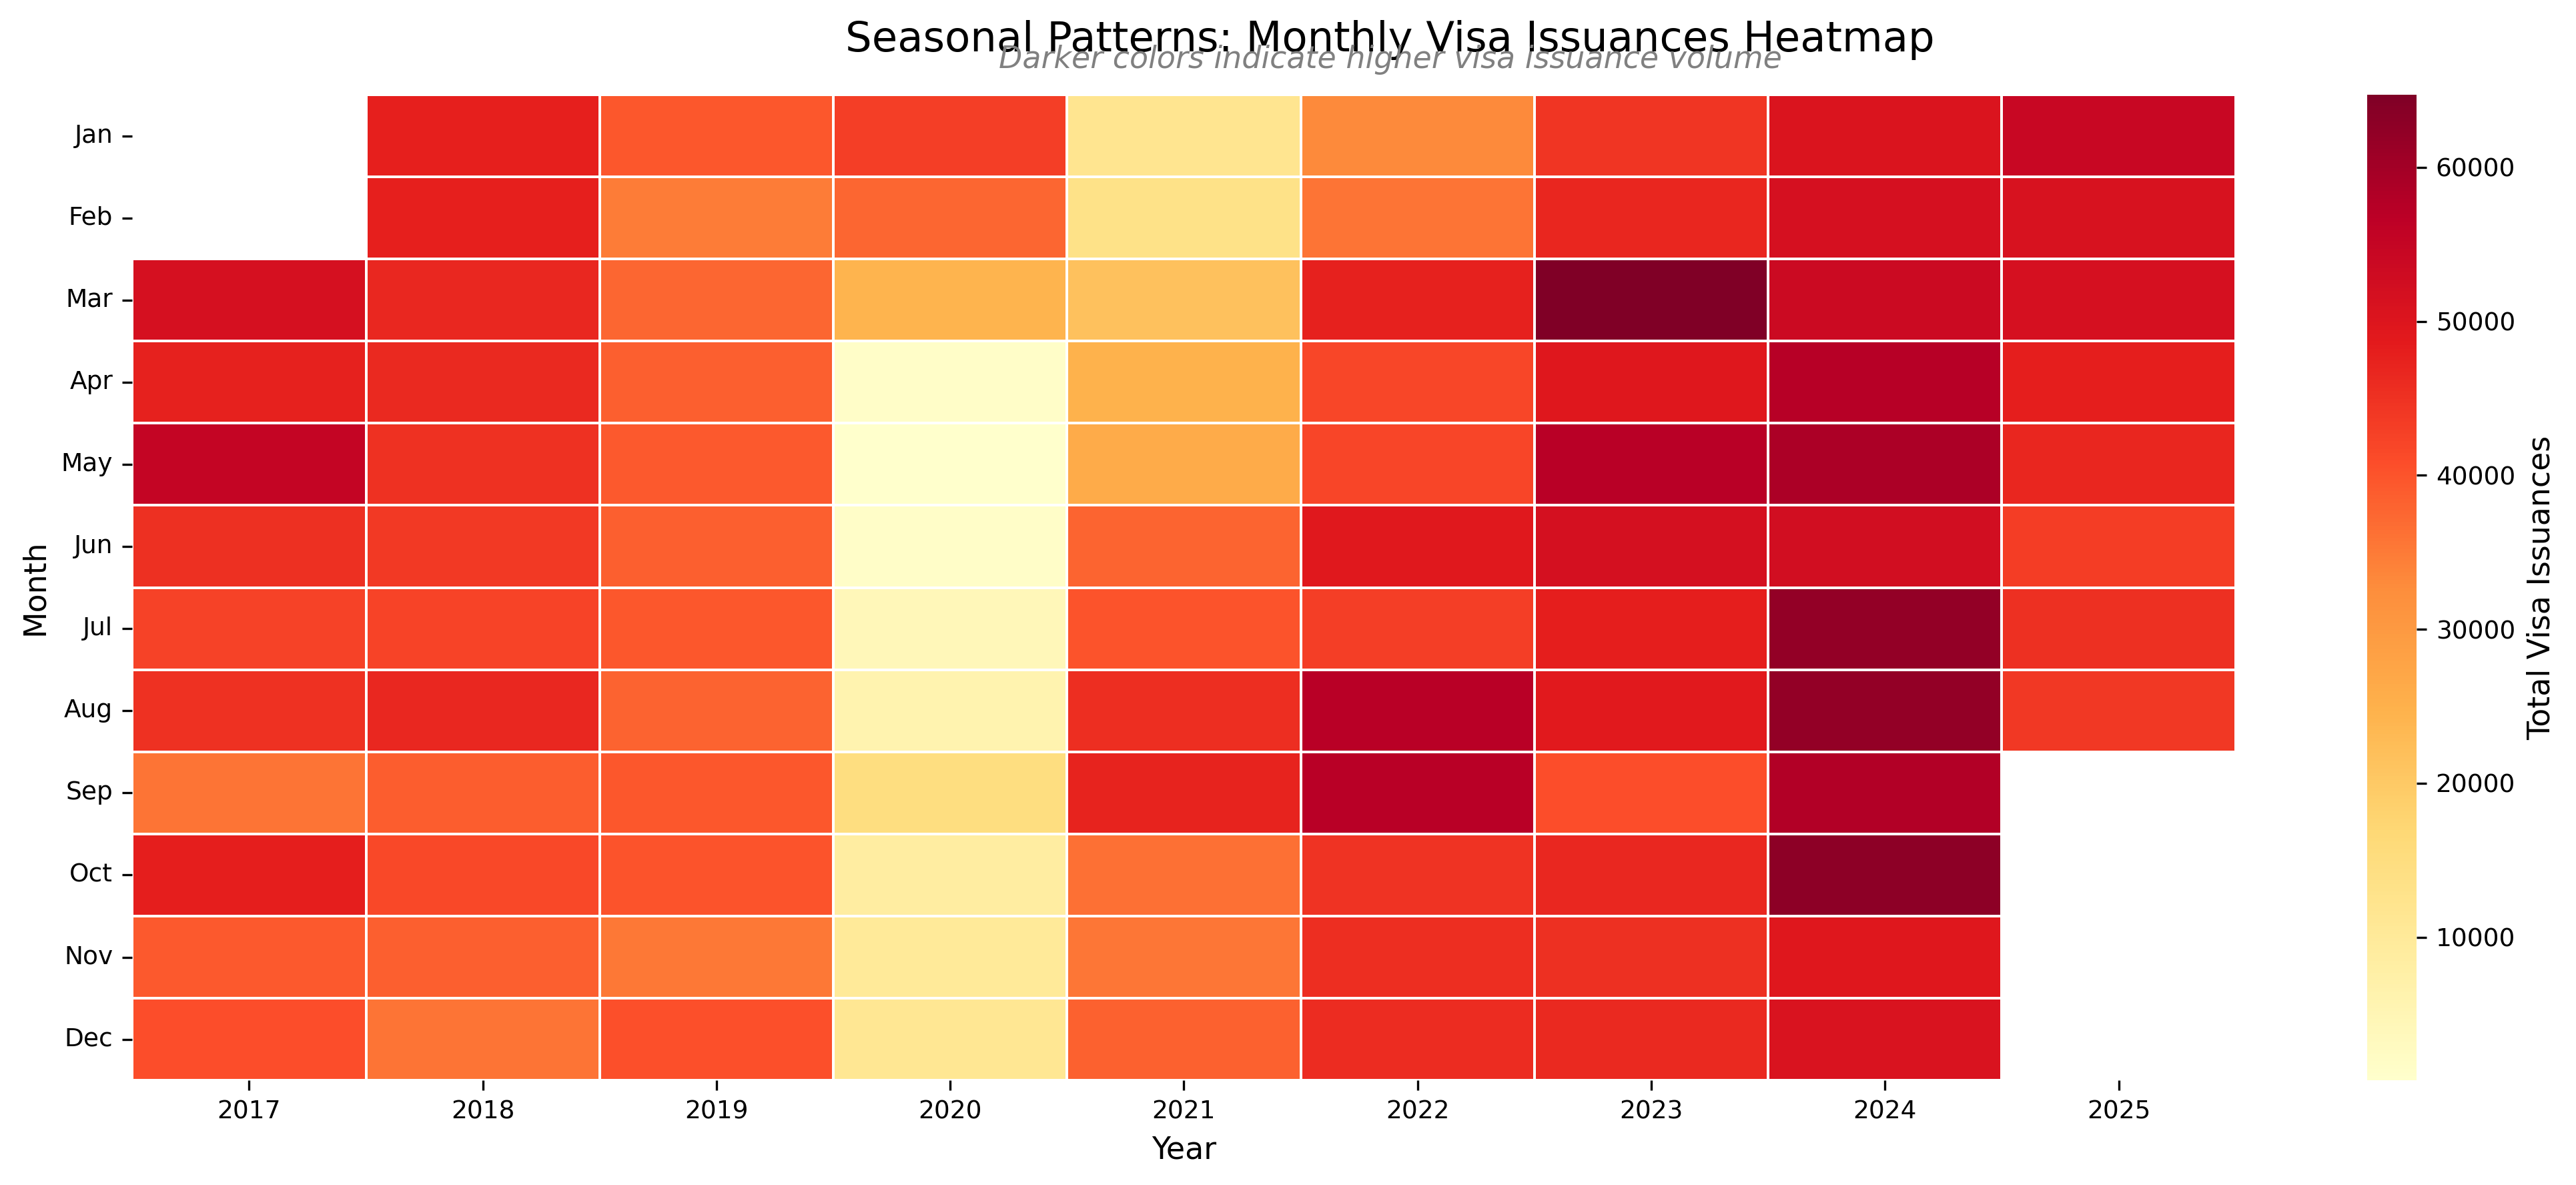
\includegraphics[width=\textwidth]{../presentation/06_seasonal_visa_heatmap_by_year.png}
  \caption{Seasonal Patterns: Monthly Visa Issuances Heatmap (2017--2025).
           Darker red shading indicates higher monthly volume.  The light-coloured
           column at 2020 reflects near-complete consulate closures during the
           COVID-19 pandemic.}
  \label{fig:seasonal_heatmap}
\end{figure}

\paragraph{Zipfian Concentration and Country Volatility.}
As noted in Section~\ref{sec:data_collection}, the cross-country distribution of
visa issuances follows a Zipfian law---the top 20\% of sending countries contribute
88.3\% of all issuances, and 81.7\% of all surge months---motivating the focus on
15 high-volume origins.  Country-level volatility, measured by the coefficient of
variation (CV) of monthly issuances, further identifies which countries are most
likely to generate abrupt surges.  As Figure~\ref{fig:visa_volatility} shows, Cuba
(CV~2.89), Afghanistan (CV~2.81), and Pakistan (CV~2.48) are the three most
volatile origins, while the Dominican Republic (CV~1.55) is comparatively stable
despite producing the strongest leading signal in the event--correlation analysis.

\begin{figure}[ht]
  \centering
  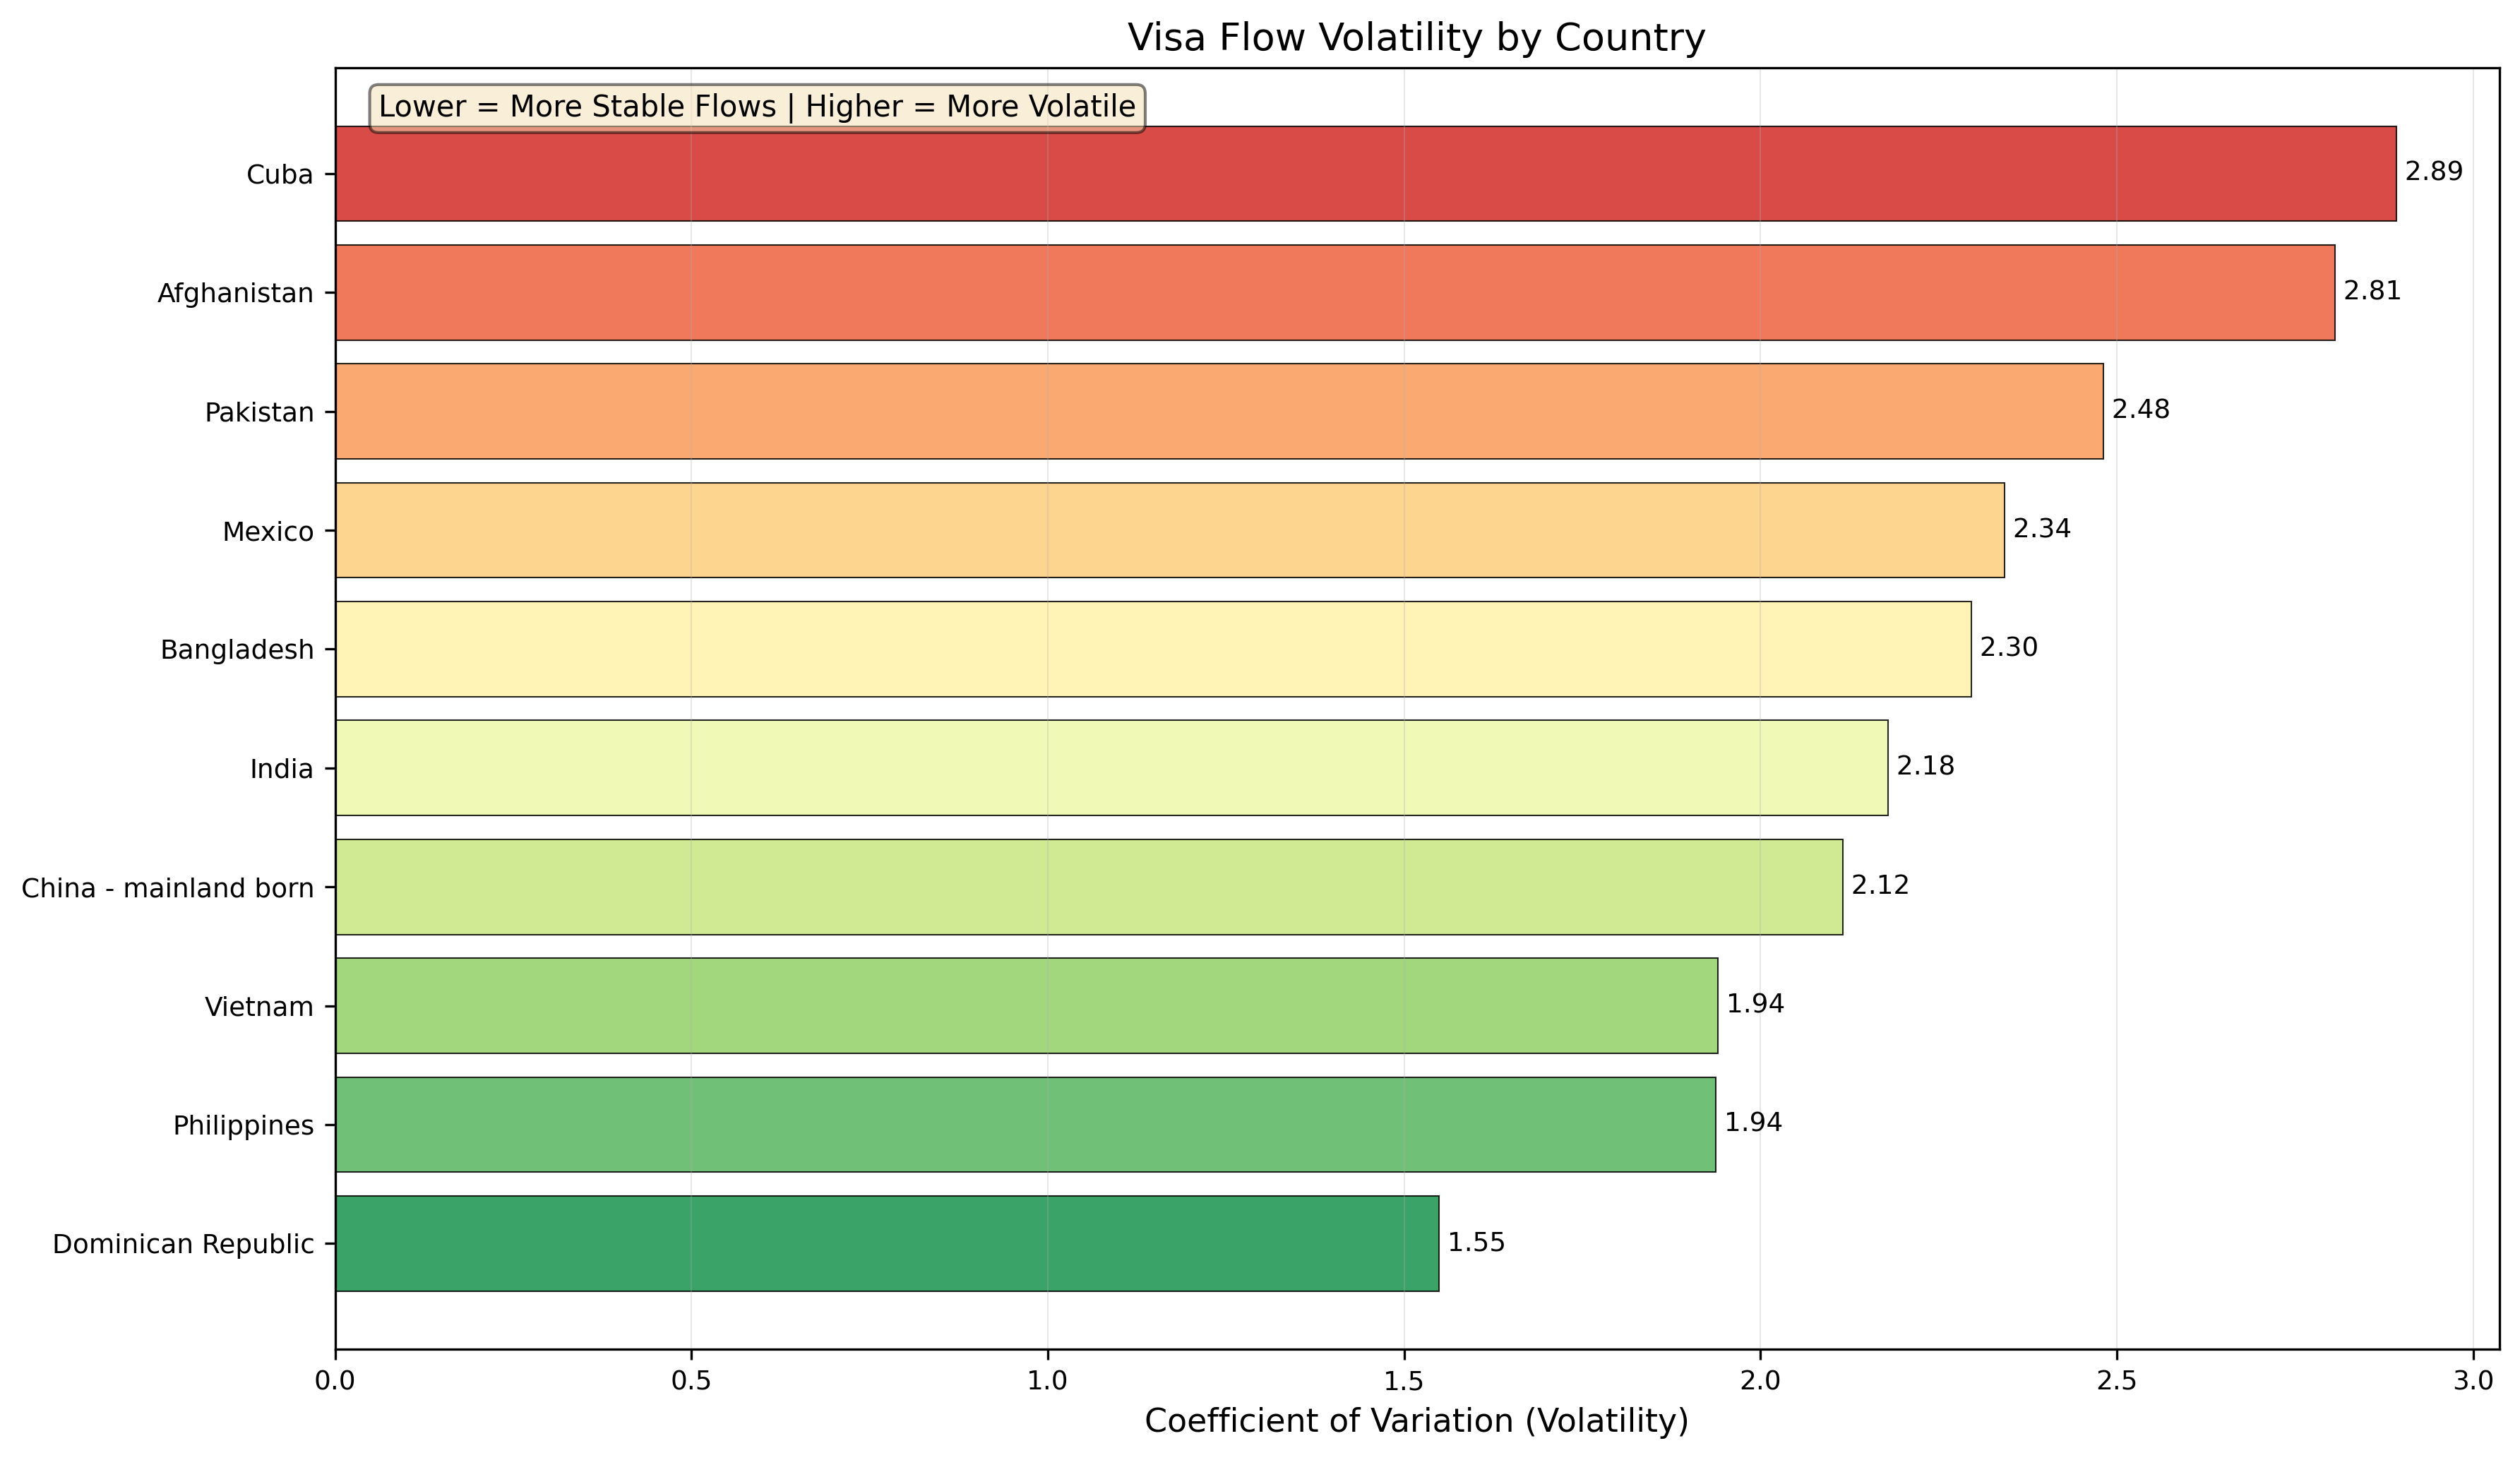
\includegraphics[width=0.87\textwidth]{../presentation/10_visa_volatility.png}
  \caption{Visa flow volatility by country, measured as the coefficient of
           variation of monthly visa issuances.  Higher values indicate more
           erratic, surge-prone flows.  Colour encodes volatility level
           (red~$=$~high, green~$=$~moderate).}
  \label{fig:visa_volatility}
\end{figure}


\subsection{Lead--Lag Signal Analysis}

For each country--signal--lag combination (lags 0--6), Pearson correlation was computed
between the signal and visa volume, with $p$-values corrected via
Benjamini--Hochberg FDR~\citep{benjamini1995} at $q \leq 0.10$.  Surge months were
defined by a dual criterion: volume above the 75th percentile \textit{or}
month-over-month growth exceeding 30\%.  Signal quality was quantified via surge
precision and surge lift.


\subsection{Predictive Models}

\paragraph{cuML Random Forest.}
A GPU-accelerated Random Forest~\citep{breiman2001,rapids_cuml} with 50 estimators and
max depth 6 served as a non-temporal baseline; six independent models were fit, one per
horizon.

\paragraph{LSTM with SurgeJointLoss.}
A two-layer LSTM~\citep{hochreiter1997} (hidden dim 64) with learned country embeddings
(dim 8) was trained with a novel dual-objective loss function, \textit{SurgeJointLoss}:
\begin{equation}
  \mathcal{L} = \alpha\;\mathcal{L}_{\mathrm{Huber}}(\hat{y},\, y)
  \;+\; (1-\alpha)\;\mathcal{L}_{\mathrm{BCE}}\!\Bigl(
    \hat{y} - \tau,\;
    \mathbf{1}\bigl[y \;>\; \mu + 1.5\,\sigma\bigr]
  \Bigr),
  \label{eq:surge_loss}
\end{equation}
where $\hat{y}$ is the predicted monthly visa volume, $y$ is the observed volume,
$\alpha = 0.6$ is a fixed mixing weight that places 60\% emphasis on volume regression
and 40\% on surge detection, $\tau$ is a learned discrimination threshold,
$\mu$ is the rolling mean of historical visa volume, $\sigma$ is its rolling standard
deviation (so $\mu + 1.5\sigma$ defines the surge boundary), $\mathcal{L}_{\mathrm{Huber}}$
is the Huber regression loss~\citep{huber1964} (robust to extreme outliers), and
$\mathcal{L}_{\mathrm{BCE}}$ is Binary Cross-Entropy applied to the surge indicator.
Both neural architectures were implemented in PyTorch~\citep{pytorch} and optimised
with Adam~\citep{kingma2015}.

\paragraph{Transformer Encoder.}
A two-layer Transformer~\citep{vaswani2017,pytorch} with 4 attention heads
($d_{\text{model}}=64$) and learnable positional encodings was trained with MSE loss as
a pure attention-based comparator.

\paragraph{Horizon-Aware Ensemble.}
The final model blends predictions from all three architectures with horizon-specific
weights that shift trust from RF/LSTM dominance at short leads toward Transformer
dominance at long leads (see Appendix~\ref{app:weights} for the full schedule).


\subsection{Validation Strategy}

All models were evaluated under a strict \textbf{walk-forward, out-of-time (OOT)}
protocol: training on data through December 2022, evaluation on 2023+.  A month-country
observation was classified as a surge if volume exceeded $1.5\sigma$ above the rolling
mean (${\sim}103$--114 surge instances in the test set).  We report Precision, Recall,
F1, and RMSE.


%% ─── Section 3: Results ──────────────────────────────────────────────────────
\section{Results}

\subsection{Multi-Signal Analysis (RQ3)}

\paragraph{News Event Signals.}
Of 392 country--event--lag combinations tested, 58 (14.8\%) achieved significance
($q \leq 0.10$).  The strongest single signal was the Dominican Republic, where a
specific cluster showed $r = 0.617$ at a 3-month lag
($q = 3.3 \times 10^{-9}$).  Cuba's ``Trump Policy'' cluster showed $r = -0.595$ at
lag~0 ($q = 3.4 \times 10^{-9}$), reflecting immediate U.S.\ policy impacts.  Eleven
of 15 countries exhibited at least one significant event signal.  Full results appear in
Appendix~\ref{app:events}.

\paragraph{Exchange Rate Signals.}
Among 6 countries with REER data, 23 of 42 lag rows (54.8\%) were significant.  The
Dominican Republic dominated ($r = 0.498$, lag~2, $q = 2.6 \times 10^{-6}$).  Overall
surge lift was modest (mean 1.009), confirming exchange rates as a complementary rather
than standalone signal.

\paragraph{Google Trends.}
Correlations were significant for 66 of 120 rows (55.0\%), but a trends-enhanced
VAR~\citep{hamilton1994,sims1980} model \textit{underperformed} the autoregressive
baseline ($-5.97\%$ mean RMSE for visas), indicating that translating keyword
correlations into out-of-sample gains requires non-linear modelling.

\paragraph{Modality Ranking.}
News event coverage emerged as the strongest individual predictor (highest single-signal
correlations, most country-specific leads); exchange rates added meaningful signal where
available (6 countries); Google Trends showed the broadest coverage but the weakest
out-of-sample translation---motivating the multi-modal fusion approach.


\subsection{Model Performance}

Table~\ref{tab:summary_perf} presents the aggregate surge-classification performance
across all six horizons.

\begin{table}[ht]
  \centering
  \caption{Average surge-classification performance (Leads 1--6, OOT test set).}
  \label{tab:summary_perf}
  \begin{tabular}{l c c c}
    \toprule
    \textbf{Algorithm} & \textbf{Precision} & \textbf{Recall} & \textbf{F1 Score} \\
    \midrule
    cuML Random Forest              & 0.870 & 0.943 & 0.907 \\
    LSTM (SurgeJointLoss)           & 0.895 & 0.820 & 0.855 \\
    Transformer Encoder             & 0.892 & 0.917 & 0.905 \\
    \textbf{Horizon-Aware Ensemble} & \textbf{0.887} & \textbf{0.943} & \textbf{0.915} \\
    \bottomrule
  \end{tabular}
\end{table}

The ensemble achieves the highest average F1 (0.915) by combining the RF's high recall
(0.943) with the Transformer's balanced precision--recall profile.  The LSTM's
conservative SurgeJointLoss objective yields the highest precision (0.895) at the cost
of lower recall (0.820).  Per-horizon breakdowns are provided in
Appendix~\ref{app:perhorizon}.

\medskip

Table~\ref{tab:rmse} reports volume prediction accuracy (RMSE) for the three base
models.

\begin{table}[ht]
  \centering
  \caption{Out-of-time RMSE by model and horizon (lower is better).
  Bold marks best per row.}
  \label{tab:rmse}
  \small
  \begin{tabular}{c c c c}
    \toprule
    \textbf{Horizon} & \textbf{Random Forest} & \textbf{Transformer} & \textbf{LSTM} \\
    \midrule
    Lead 1 & 298.79 & 303.43 & \textbf{277.40} \\
    Lead 2 & 341.79 & 343.61 & \textbf{320.77} \\
    Lead 3 & 351.55 & 359.20 & \textbf{346.03} \\
    Lead 4 & \textbf{364.01} & 381.20 & 381.00 \\
    Lead 5 & 428.35 & 407.67 & \textbf{404.23} \\
    Lead 6 & \textbf{401.38} & 426.48 & 424.59 \\
    \bottomrule
  \end{tabular}
\end{table}

The LSTM dominates near-term volume prediction (Leads 1--3) by 10--20 RMSE points; at
longer horizons the RF maintains competitive parity.


\subsection{Architecture Insights (RQ2)}

\begin{enumerate}
  \item \textbf{Random Forest:} highest single-model F1 at Lead~1 (0.97) and recall of
        0.943 on average, but precision degrades at longer horizons.
  \item \textbf{LSTM:} highest precision (0.895 average) thanks to SurgeJointLoss---when
        it fires an alarm, it is the most likely to be genuine.  The trade-off is lower
        recall (0.820).
  \item \textbf{Transformer:} superior long-horizon recall (90\% at Lead~6) and the
        highest individual-model F1 at Lead~6 (0.87), capturing slow geopolitical
        dynamics via self-attention.
  \item \textbf{Ensemble:} by shifting trust from RF/LSTM at short leads toward the
        Transformer at long leads, it achieves the best F1 at every horizon and
        maintains \textbf{recall $\geq 0.92$} across all six months.
\end{enumerate}


%% ─── Section 4: Conclusion ─────────────────────────────────────────────────
\section{Conclusion}

This study has demonstrated that multi-modal digital trace data---when processed
through architectures designed to capture surge dynamics---can reliably anticipate
migration crises months before they materialise.  Across all three research questions
the evidence converges on a clear answer: fusing news event coverage, search-intent
signals, and macroeconomic indicators into a Horizon-Aware Ensemble yields consistent
gains over every single-modality or single-architecture baseline, with the ensemble
achieving an average F1 of 0.915 and recall $\geq 0.92$ at every forecast horizon
from one to six months.  These results indicate that the ``precision blindspot''
afflicting traditional reactive migration management is not an inherent feature of the
forecasting problem, but an artefact of relying on slow-moving aggregate statistics
rather than the rich signal landscape now observable through digital sources.
Pre-emptive planning---staffing adjustments, logistics pre-positioning, diplomatic
engagement---becomes tractable when high-recall early warnings arrive months in advance.

\subsection{Practical Implications}

\begin{itemize}
  \item \textbf{Lead 1 (F1 0.96):} Immigration processing centres can adjust staffing
        for the coming month with high confidence.
  \item \textbf{Lead 3 (F1 0.93):} Humanitarian organisations can pre-position
        supplies and shelter capacity in anticipated surge corridors.
  \item \textbf{Lead 6 (F1 0.86):} National-level budgetary and diplomatic planning
        can be initiated with sufficient institutional lead time.
\end{itemize}

The finding that news event signals around U.S.\ policy announcements serve as the
strongest leading indicators suggests that \textbf{monitoring origin-country media
coverage could function as a low-cost early warning input} even without sophisticated
modelling infrastructure.

\subsection{Limitations}

\paragraph{The Digital Divide.}
Google Trends and digital news reflect populations with internet access.
The most vulnerable migrants---those displaced by conflict or extreme poverty in regions
with limited digital infrastructure---may be systematically underrepresented, creating a
blind spot for the most acutely at-risk groups.

\paragraph{Correlation, Not Causation.}
This is a \textit{predictive} model, not a \textit{causal} one.  Lead--lag correlations
identify temporal associations, but establishing causal mechanisms would require
quasi-experimental or instrumental-variable approaches outside the present scope.

\paragraph{Exchange Rate Data Gap.}
REER data was available for only 6 of 15 target countries~\citep{imf_reer}, excluding
high-priority origins (Afghanistan, Cuba, Haiti, Honduras, Venezuela, among others).

\paragraph{Black Swan Events.}
Genuinely novel shocks---sudden asylum-law changes, region-scale disasters, unprecedented
policy events---lie beyond the model's anticipatory reach.  The system should complement,
not replace, domain expert judgement.  Five additional limitations are discussed in
Appendix~\ref{app:limitations}.\label{sec:limitations}


\subsection{Future Work}

Key extensions include social media integration for finer-grained intent signals,
cross-country transfer learning from data-rich to data-sparse origins, real-time
streaming deployment, and causal discovery via Granger causality or structural equation
models.  See Appendix~\ref{app:futurework} for the full enumeration.

\subsection{Code and Data Availability}

The full codebase, including data-collection scripts, model implementations, and
reproduction notebooks, is publicly available at
\url{https://github.com/ibitec7/migration}.  Pre-trained model weights, processed
datasets, and intermediate artefacts (embeddings, cluster labels, production outputs)
are hosted on Hugging Face at \url{https://huggingface.co/sdsc2005-migration}.


%% ─── Section 5: Contribution Statement ──────────────────────────────────────
\section{Contribution Statement}

\begin{itemize}
  \item \textbf{Ibrahim:} Multi-modal data ingestion pipeline (async news scraping of
        170K+ articles, Trends collection, HF data sync, data processing).
  \item \textbf{Haseeb:} LSTM and Transformer architectures, SurgeJointLoss
        implementation, model performance visualisations.
  \item \textbf{Asadohoo:} News scraping, URL decoding pipeline, NLP processing
        (embeddings, clustering, headline scoring).
  \item \textbf{Sameer:} Exploratory data analysis on encounter and visa data
        (Zipfian analysis, seasonal decomposition), Introduction drafting.
  \item \textbf{Ayaan:} Horizon-Aware Ensemble, per-horizon surge metrics, lead--lag signal analysis across modalities.
  \item \textbf{Pak Hei Ng:} cuML Random Forest baseline, GPU-accelerated clustering,
        report aggregation, formatting, and references.
\end{itemize}


%% ─── References ──────────────────────────────────────────────────────────────
\newpage
\bibliographystyle{plainnat}
\bibliography{references}


%% ═════════════════════════════════════════════════════════════════════════════
%%  APPENDIX
%% ═════════════════════════════════════════════════════════════════════════════
\newpage
\begin{appendices}

%% ─── Appendix A ──────────────────────────────────────────────────────────────
\section{Per-Horizon Surge Classification}\label{app:perhorizon}

The summary Table~\ref{tab:summary_perf} in the main body reports averages across
horizons.  Tables~\ref{tab:rf_class}--\ref{tab:ens_class} below provide the full
break-down for each model on the OOT test set (${{\sim}103}$--114 surge instances,
threshold $> 1.5\sigma$).  The consistent decline in metrics from Lead~1 to Lead~6
reflects the difficulty of long-range forecasting; the ensemble mitigates this decay
more effectively than any individual model.

\begin{table}[ht]
  \centering
  \caption{Random Forest surge classification (OOT).}
  \label{tab:rf_class}
  \small
  \begin{tabular}{c c c c}
    \toprule
    \textbf{Horizon} & \textbf{Prec.} & \textbf{Rec.} & \textbf{F1} \\
    \midrule
    Lead 1 & 0.96 & 0.97 & \textbf{0.97} \\
    Lead 2 & 0.93 & 0.95 & \textbf{0.94} \\
    Lead 3 & 0.88 & 0.96 & \textbf{0.92} \\
    Lead 4 & 0.85 & 0.94 & \textbf{0.89} \\
    Lead 5 & 0.82 & 0.93 & \textbf{0.88} \\
    Lead 6 & 0.78 & 0.91 & \textbf{0.84} \\
    \bottomrule
  \end{tabular}
\end{table}

\begin{table}[ht]
  \centering
  \caption{Transformer Encoder surge classification (OOT).}
  \label{tab:trans_class}
  \small
  \begin{tabular}{c c c c}
    \toprule
    \textbf{Horizon} & \textbf{Prec.} & \textbf{Rec.} & \textbf{F1} \\
    \midrule
    Lead 1 & 0.95 & 0.93 & \textbf{0.94} \\
    Lead 2 & 0.95 & 0.94 & \textbf{0.94} \\
    Lead 3 & 0.91 & 0.93 & \textbf{0.92} \\
    Lead 4 & 0.86 & 0.90 & \textbf{0.88} \\
    Lead 5 & 0.85 & 0.90 & \textbf{0.88} \\
    Lead 6 & 0.83 & 0.90 & \textbf{0.87} \\
    \bottomrule
  \end{tabular}
\end{table}

\begin{table}[ht]
  \centering
  \caption{LSTM (SurgeJointLoss) surge classification (OOT).}
  \label{tab:lstm_class}
  \small
  \begin{tabular}{c c c c}
    \toprule
    \textbf{Horizon} & \textbf{Prec.} & \textbf{Rec.} & \textbf{F1} \\
    \midrule
    Lead 1 & 0.97 & 0.85 & \textbf{0.91} \\
    Lead 2 & 0.94 & 0.84 & \textbf{0.89} \\
    Lead 3 & 0.91 & 0.83 & \textbf{0.87} \\
    Lead 4 & 0.88 & 0.81 & \textbf{0.84} \\
    Lead 5 & 0.85 & 0.80 & \textbf{0.82} \\
    Lead 6 & 0.82 & 0.79 & \textbf{0.80} \\
    \bottomrule
  \end{tabular}
\end{table}

\begin{table}[ht]
  \centering
  \caption{Horizon-Aware Ensemble surge classification (OOT).}
  \label{tab:ens_class}
  \small
  \begin{tabular}{c c c c}
    \toprule
    \textbf{Horizon} & \textbf{Prec.} & \textbf{Rec.} & \textbf{F1} \\
    \midrule
    Lead 1 & 0.96 & 0.96 & \textbf{0.96} \\
    Lead 2 & 0.93 & 0.96 & \textbf{0.95} \\
    Lead 3 & 0.92 & 0.94 & \textbf{0.93} \\
    Lead 4 & 0.88 & 0.94 & \textbf{0.91} \\
    Lead 5 & 0.83 & 0.94 & \textbf{0.88} \\
    Lead 6 & 0.80 & 0.92 & \textbf{0.86} \\
    \bottomrule
  \end{tabular}
\end{table}


%% ─── Appendix B ──────────────────────────────────────────────────────────────
\section{Detailed Event Signal Analysis}\label{app:events}

Of 392 country--event--lag combinations screened, 58 (14.8\%) survived
Benjamini--Hochberg correction at $q \leq 0.10$.  Selected highlights across
modalities are described below.

\paragraph{News event clusters.}
Among cluster-level signals, Mexico's geopolitical-watch cluster showed
$r = -0.436$ at a 1-month lag ($q = 0.0009$), India's economic-sentiment cluster
showed $r = -0.424$ at 2~months ($q = 0.0010$, surge lift 0.932), Honduras's
Evangelical-pastoral cluster showed $r = +0.327$ at 2~months ($q = 0.0114$,
lift 1.229), Vietnam's misinformation cluster showed $r = -0.403$ at 5~months
($q = 0.0017$, lift 0.816), and El~Salvador's conflict cluster showed $r = -0.361$
at 5~months ($q = 0.0055$, lift 0.842).  Eleven of the 15 countries exhibited at
least one significant event signal.

\paragraph{Headline sentiment scores.}
Aggregate headline-level scores revealed sharper relationships still.  The
Dominican Republic produced the single strongest lead in the study: $r = 0.617$ at
a 3-month lag ($q = 3.3 \times 10^{-9}$).  Cuba's ``Trump Policy'' cluster showed
$r = -0.595$ at lag~0 ($q = 3.4 \times 10^{-9}$), capturing the immediate visa
impact of U.S.\ policy shifts.

\paragraph{Exchange rate and Trends signals.}
Among the 6 countries with REER data, the Dominican Republic again dominated
($r = 0.498$, lag~2, $q = 2.6 \times 10^{-6}$), followed by Mexico ($r = 0.289$,
lag~6, $q = 0.018$).  Google Trends was significant for 66 of 120 rows (55.0\%);
notable examples include China's \texttt{us\_visa} keyword ($r = 0.406$,
$q = 1.1 \times 10^{-4}$) and Afghanistan's \texttt{us\_jobs} ($r = -0.484$,
$q = 4.4 \times 10^{-6}$).


%% ─── Appendix C ──────────────────────────────────────────────────────────────
\section{Extended Limitations}\label{app:limitations}

The following supplement the four limitations discussed in the Conclusion (§4.2).

\paragraph{Google Trends as a Weak Standalone Predictor.}
Despite significant keyword-level correlations, the trends-enhanced VAR model
underperformed the autoregressive baseline ($-5.97\%$ RMSE on average), indicating that
search-intent signals require non-linear architectures to be leveraged effectively.

\paragraph{News Coverage Bias.}
The 61.1\% pipeline success rate means roughly 39\% of articles were lost to extraction
failures, paywalls, or anti-scraping measures.  Coverage is skewed toward
English-language media, potentially underrepresenting local-language reporting.

\paragraph{Feature Interpretability and Selective Collection.}
Random Forest feature importance scores are currently unused for guiding data
collection.  Systematic importance analysis could concentrate future efforts on
high-signal inputs, reducing operational cost.

\paragraph{Model Staleness and Distributional Drift.}
The model is anchored to the 2017--2022 training window.  Concept drift---particularly
shifts in the Zipfian distribution of visa issuances as geopolitical pressures evolve
---could push the system out-of-distribution without periodic retraining.

\paragraph{Survivorship Bias in Encounter Data.}
Border encounters record only \textit{detected} crossings; migrants who evade
apprehension are absent.  The model therefore partially learns enforcement detection
rates rather than true migration pressure.


%% ─── Appendix D ──────────────────────────────────────────────────────────────
\section{Ensemble Weight Schedule}\label{app:weights}

Table~\ref{tab:ensemble_weights} shows the horizon-specific weighting scheme.

\begin{table}[ht]
  \centering
  \caption{Horizon-Aware Ensemble weights (sum to 1.0 per row).}
  \label{tab:ensemble_weights}
  \small
  \begin{tabular}{c c c c p{4.8cm}}
    \toprule
    \textbf{Lead} & \textbf{RF} & \textbf{Trans.} & \textbf{LSTM} &
    \textbf{Rationale} \\
    \midrule
    1\,mo & 60\% & 10\% & 30\% & RF \& LSTM dominate short-term \\
    2\,mo & 50\% & 20\% & 30\% & RF still dominant \\
    3\,mo & 30\% & 40\% & 30\% & Balanced transition \\
    4\,mo & 20\% & 60\% & 20\% & Transformer increasingly critical \\
    5\,mo & 10\% & 80\% & 10\% & Transformer dominates long-horizon \\
    6\,mo &  5\% & 85\% & 10\% & Transformer captures slow trends \\
    \bottomrule
  \end{tabular}
\end{table}


%% ─── Appendix E ──────────────────────────────────────────────────────────────
\section{Future Work}\label{app:futurework}

\begin{enumerate}
  \item \textbf{Social media integration:} Signals from X (Twitter), Facebook, and
        WhatsApp could provide finer-grained, less media-filtered insight into
        migration intent.
  \item \textbf{Cross-country transfer learning:} Training on data-rich countries
        (Mexico, India) and transferring representations to data-sparse origins (Haiti,
        Afghanistan).
  \item \textbf{Real-time streaming:} Adapting the batch-monthly pipeline for
        continuous ingestion with rolling daily or weekly forecasts.
  \item \textbf{Richer macro indicators:} Incorporating inflation, unemployment,
        remittance flows, and commodity prices to fill exchange-rate gaps.
  \item \textbf{Causal discovery:} Applying Granger causality, structural equation
        models, or natural-experiment designs to move beyond predictive correlation.
\end{enumerate}


%% ─── Appendix F ──────────────────────────────────────────────────────────────
\section{Data Pipeline Engineering Details}\label{app:pipeline}

The news collection pipeline was engineered for throughput and fault tolerance:

\begin{itemize}
  \item Articles were collected via the Google News RSS API~\citep{google_news}, with
        encoded URLs resolved through a batched decoding endpoint (20 articles per
        batch), reducing API calls by ${\sim}$95\%.
  \item Full article text was fetched asynchronously with semaphore-controlled
        concurrency (max 16 connections), exponential backoff with jitter, and a
        30-second watchdog timeout per request.
  \item HTML-to-text extraction was performed via
        Trafilatura~\citep{trafilatura}, parallelized across CPU cores using a
        \texttt{ProcessPoolExecutor} (4~workers).
  \item Intermediate results were checkpointed every 25 articles via atomic writes
        (write to temp file, then rename), ensuring crash-resilient resumption.
\end{itemize}

Exploratory and model-performance plots (visa time series, encounter trends,
cluster UMAP visualisations, F1 trajectory charts, and lead--lag heatmaps) are
stored in the \texttt{data/plots/} directory of the project repository, organised
into sub-folders: \texttt{eda\_plots/}, \texttt{cluster\_plots/},
\texttt{model\_performance/}, and \texttt{trends\_vs\_migration/}.


%% ─── Appendix G ──────────────────────────────────────────────────────────────
\section{Cluster Quality Analysis}\label{app:clusterquality}

Figures~\ref{fig:silhouette} and~\ref{fig:unique_clusters} summarise the quality
and thematic granularity of the HDBSCAN event clusters produced for each of the
15 origin countries.

\paragraph{Silhouette Scores.}
A silhouette score above 0.5 indicates well-separated, internally coherent
clusters.  As Figure~\ref{fig:silhouette} shows, the majority of countries achieve
scores above this threshold; the United States (US-centric context articles),
China, and the Philippines reach 0.70--0.82, confirming that Jina~v5 embeddings
capture thematically distinct news groupings.  Cuba and Colombia are the notable
exceptions (scores 0.28--0.43), reflecting noisier or more topically overlapping
news coverage for those origins.

\begin{figure}[ht]
  \centering
  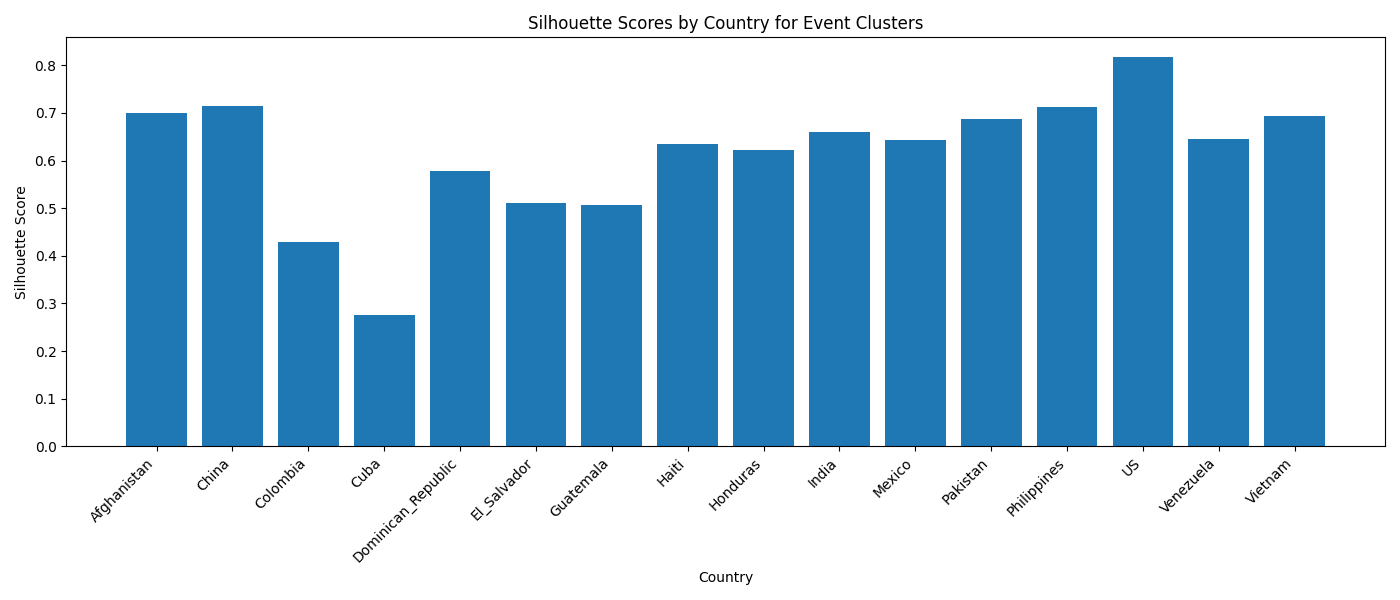
\includegraphics[width=\textwidth]{../presentation/silhouette_scores_by_country.png}
  \caption{Silhouette scores by country for HDBSCAN event clusters.  Values
           above 0.5 indicate well-separated, internally coherent clusters.
           Most countries exceed this threshold, validating the Jina~v5 embedding
           space as a meaningful basis for thematic grouping.}
  \label{fig:silhouette}
\end{figure}

\paragraph{Number of Unique Clusters.}
Figure~\ref{fig:unique_clusters} shows that Cuba, El~Salvador, and Guatemala
produced the largest number of distinct event themes (6~clusters each), reflecting
richer and more varied news landscapes for these countries in the context of
U.S.\ migration.  Countries with fewer clusters (3) such as Afghanistan, Colombia,
and India tended to have more concentrated coverage around a single dominant
narrative (e.g., Taliban governance or H-1B visa policy), which can make cluster
labels simpler but potentially reduces signal diversity.

\begin{figure}[ht]
  \centering
  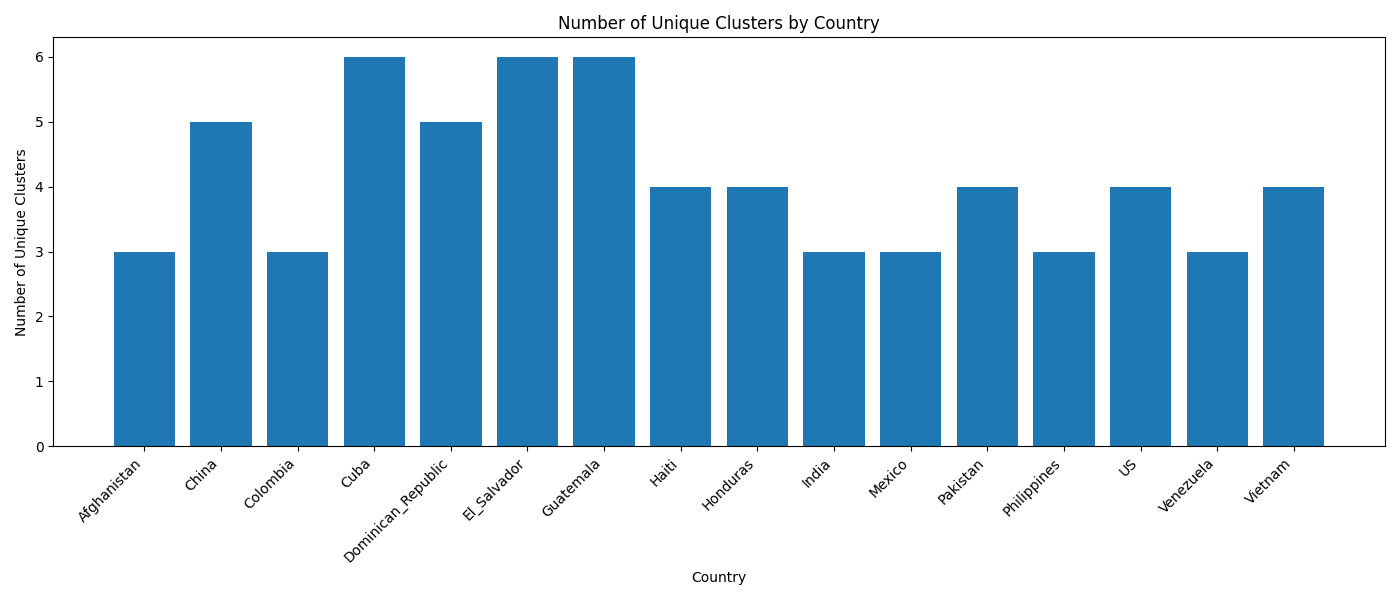
\includegraphics[width=\textwidth]{../presentation/unique_clusters_by_country.png}
  \caption{Number of unique HDBSCAN event clusters per country.  Greater cluster
           counts indicate richer thematic diversity in the collected news corpus,
           providing more candidate leading indicators per origin.}
  \label{fig:unique_clusters}
\end{figure}


%% ─── Appendix H ──────────────────────────────────────────────────────────────
\section{F1-Score Trajectory Across Forecast Horizons}\label{app:f1horizon}

Figure~\ref{fig:f1_horizon} plots per-lead F1~scores for all four models on the
OOT test set, complementing the tabular summaries in
Tables~\ref{tab:rf_class}--\ref{tab:ens_class} and giving an at-a-glance view of
how each architecture's surge-detection ability degrades with forecast distance.

\begin{figure}[ht]
  \centering
  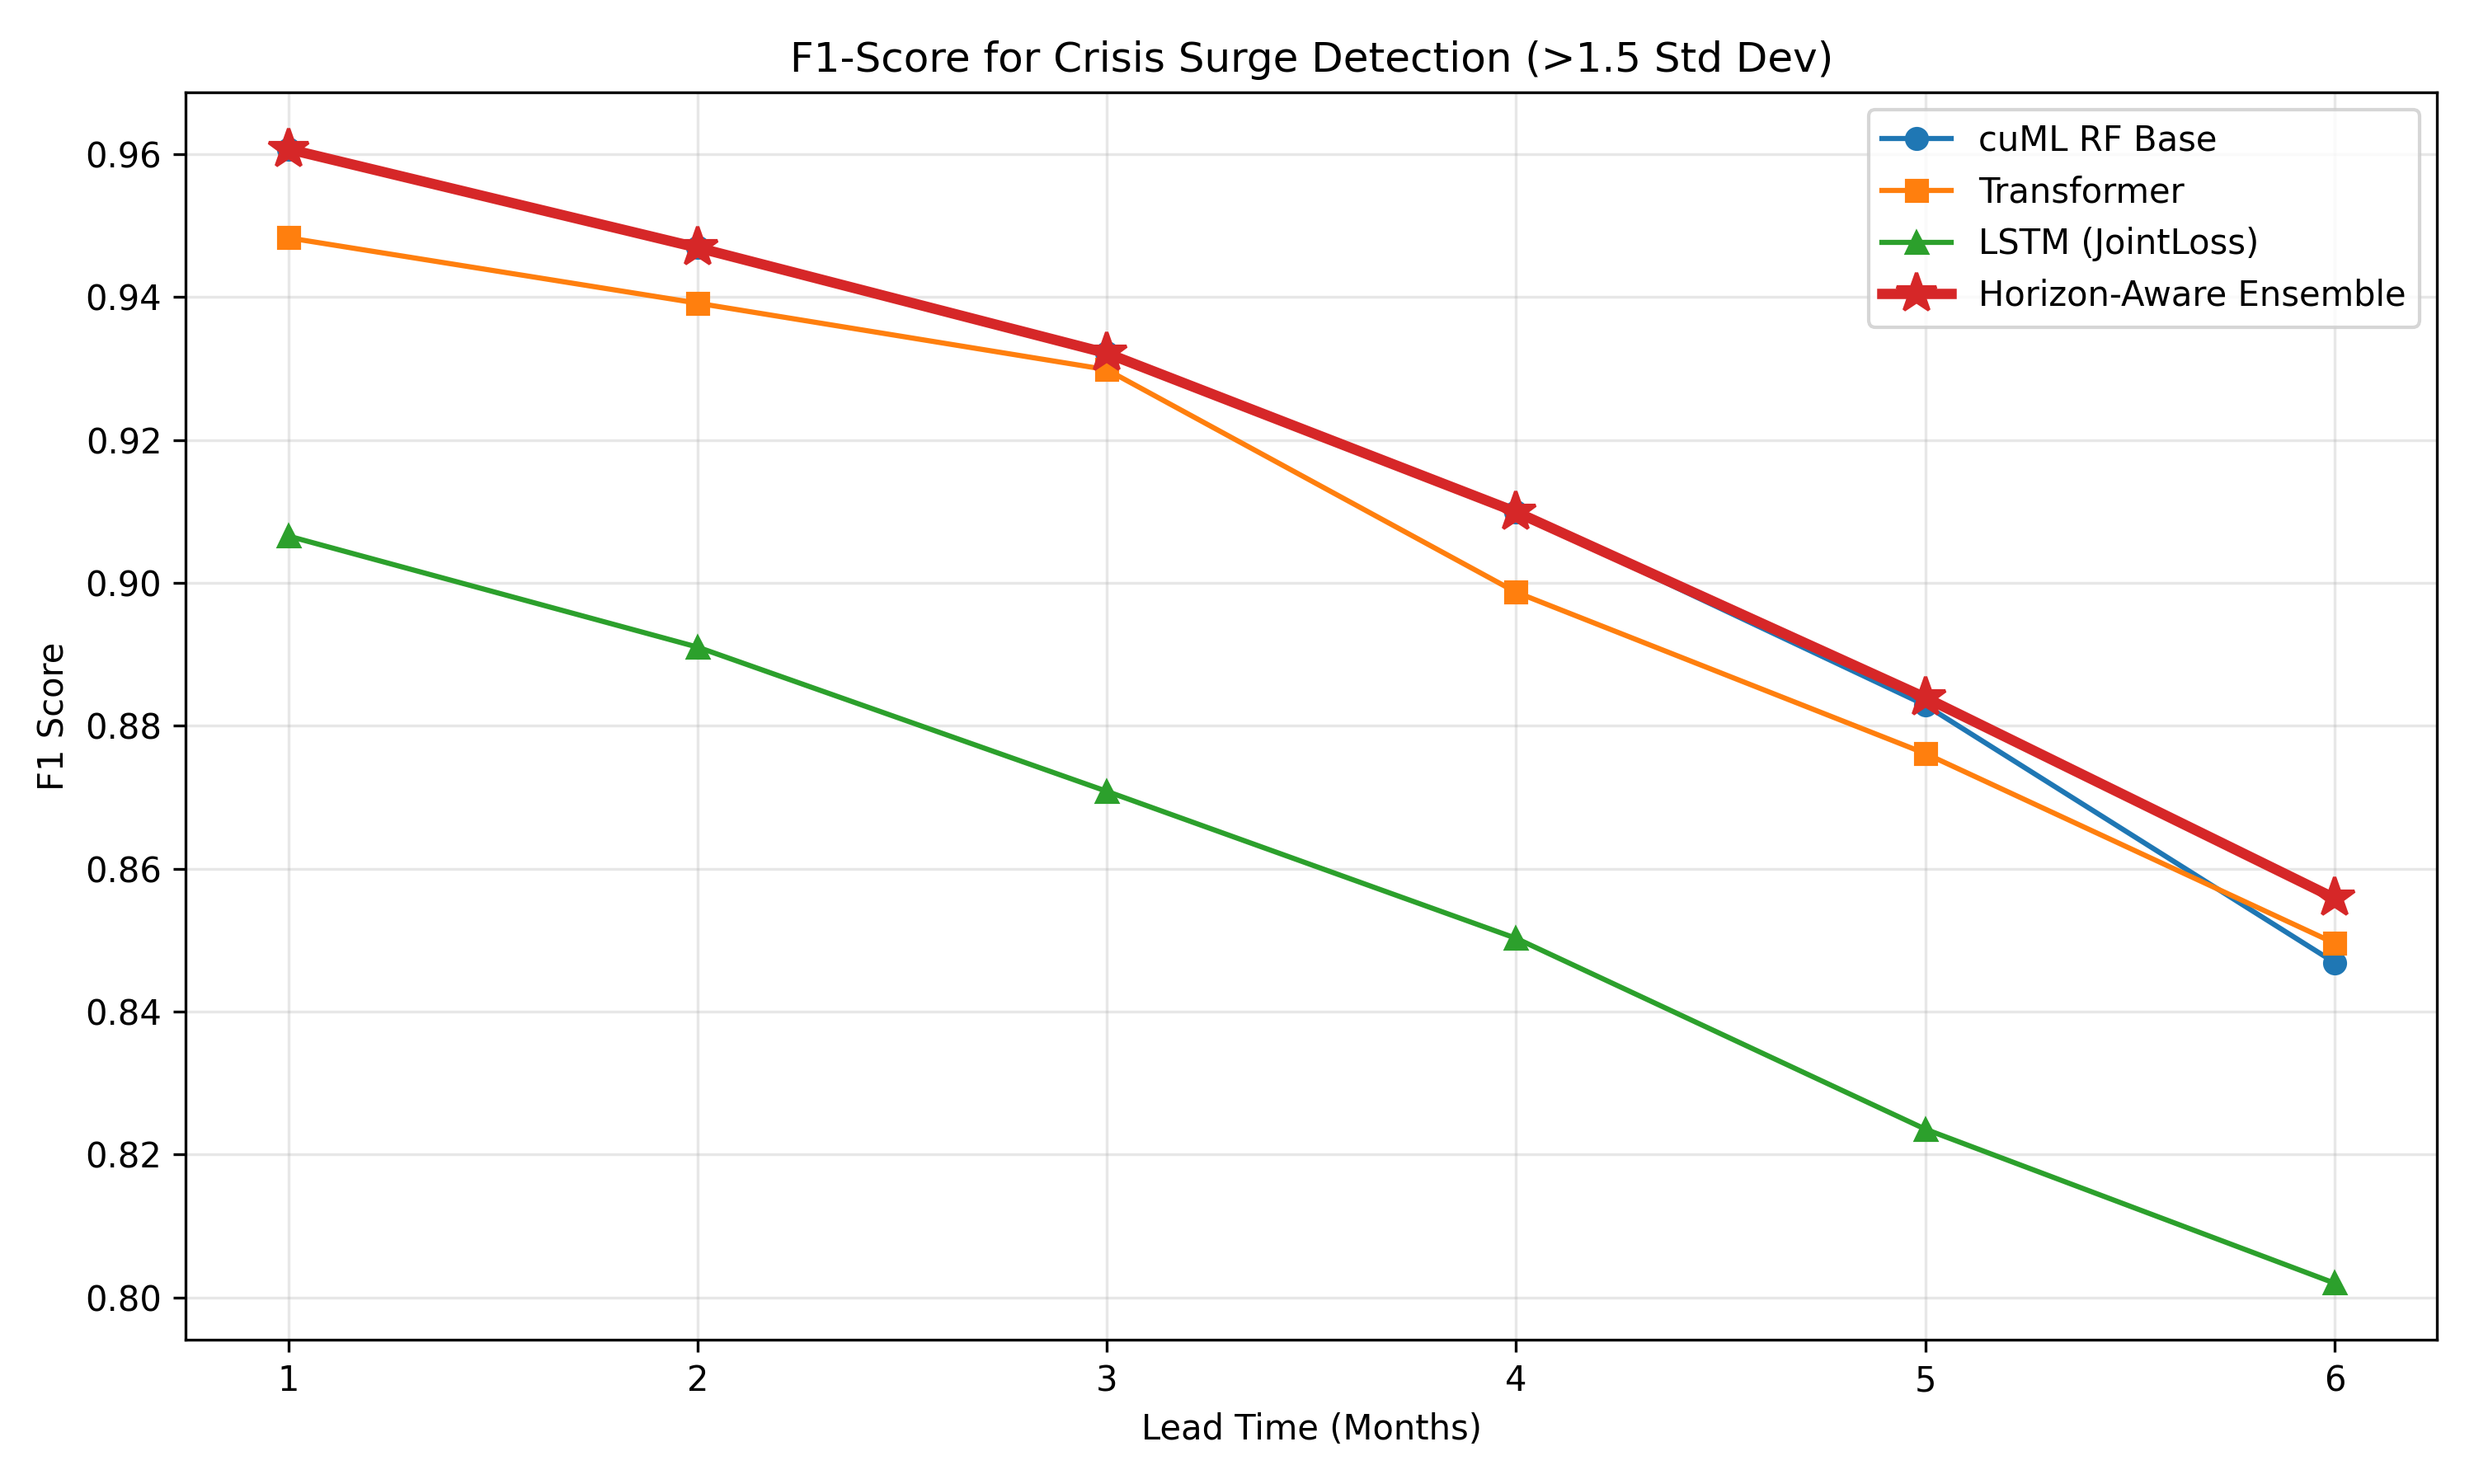
\includegraphics[width=\textwidth]{../presentation/f1_score_by_horizon.png}
  \caption{F1 scores for surge detection across forecast lead times (Leads 1--6).
           All models degrade with increasing horizon; the Horizon-Aware Ensemble
           (red star) consistently outperforms individual architectures at every
           lead.  The LSTM (JointLoss, green triangle) trades lower F1 for higher
           precision, visible as the most conservative trajectory.}
  \label{fig:f1_horizon}
\end{figure}

The ensemble curve is notably flatter than that of any individual model, confirming
that the horizon-specific weighting schedule (Appendix~\ref{app:weights})
successfully compensates for the complementary decay profiles of Random Forest and
Transformer.  The Horizon-Aware Ensemble maintains F1~$>0.86$ even at Lead~6---a
2-percentage-point improvement over the best single model at that horizon.

\end{appendices}
\end{document}
